\documentclass[sectionlevel=book]{noteformyself}


% need \usepackage{unicode-math} in preamble

%一些常用的宏定义
\newcommand{\kk}{{\symbf{k}}}
\newcommand{\kkk}{{\mathbb{k}}}
\newcommand{\KK}{{\symbf{K}}}
\newcommand{\KKK}{{\mathbb{K}}}
\newcommand{\rkk}{{\kappa}} % residue field
\newcommand{\fkk}{{\mathscr{K}}} % fraction field

\renewcommand{\d}{{\symrm{d}}}
\renewcommand{\i}{{\symrm{i}}}
\renewcommand{\P}{\partial}


% for category theory
\newcommand{\Set}{\symbf{Set}}
\newcommand{\Var}{\symbf{Var}}
\newcommand{\Sch}{\symbf{Sch}}
\newcommand{\Alg}{\symbf{Alg}}
\newcommand{\Ring}{\symbf{Ring}}
\newcommand{\Mod}{\symbf{Mod}}
\newcommand{\TopMod}{\symbf{TopMod}}
\newcommand{\Grp}{\symbf{Grp}}
\newcommand{\Ab}{\symbf{Ab}}
\newcommand{\Top}{\symbf{Top}}
\newcommand{\Cat}{\symbf{Cat}}
\newcommand{\AlgSp}{\symbf{AlgSp}}
\newcommand{\Obj}{\operatorname{Obj}}


\newcommand{\ten}{\otimes}
\newcommand{\ratmap}{\dasharrow}
\newcommand{\injmap}{\hookrightarrow}
\newcommand{\surjmap}{\twoheadrightarrow}

\newcommand{\invlim}{\varprojlim}
\newcommand{\dirlim}{\varinjlim}

\newcommand{\id}{{\operatorname{id}}}

\newcommand{\Frac}{\operatorname{Frac}}
\newcommand{\Der}{\operatorname{Der}}
\newcommand{\Spec}{\operatorname{Spec}}
\newcommand{\Proj}{\operatorname{Proj}}
\newcommand{\mSpec}{\operatorname{mSpec}}
\newcommand{\depth}{\operatorname{depth}}
\newcommand{\idealht}{\operatorname{ht}}
\newcommand{\codim}{\operatorname{codim}}
\newcommand{\Supp}{\operatorname{Supp}}
\newcommand{\trdeg}{\operatorname{trdeg}}
\newcommand{\Ass}{\operatorname{Ass}}
\newcommand{\Ann}{\operatorname{Ann}}
\newcommand{\Ext}{\operatorname{Ext}}
\newcommand{\Tor}{\operatorname{Tor}}
\newcommand{\Hom}{\operatorname{Hom}}
\newcommand{\Eq}{\operatorname{Eq}}
\newcommand{\End}{\operatorname{End}}
\newcommand{\Mor}{\operatorname{Mor}}
\newcommand{\Mult}{\operatorname{Mult}}
\newcommand{\Image}{\operatorname{Im}}
\newcommand{\Ker}{\operatorname{Ker}}
\newcommand{\coker}{\operatorname{coker}}
\newcommand{\rank}{\operatorname{rank}}
\newcommand{\cohdim}{\operatorname{coh.dim}}
\newcommand{\hldim}{\operatorname{hl.dim}}
\newcommand{\projdim}{\operatorname{proj.dim}}
\newcommand{\injdim}{\operatorname{inj.dim}}
\newcommand{\rad}{\operatorname{rad}}
\newcommand{\nil}{\operatorname{nil}}
\newcommand{\characteristic}{\operatorname{char}}
\newcommand{\Pic}{\operatorname{Pic}}
\newcommand{\NS}{\operatorname{NS}}
\newcommand{\Exc}{\operatorname{Exc}}
\newcommand{\Sing}{\operatorname{Sing}}
\newcommand{\Bl}{\operatorname{Bl}}
\newcommand{\Reg}{\operatorname{Reg}}
\newcommand{\Tr}{\operatorname{Tr}}
\newcommand{\Psef}{\operatorname{Psef}}
\newcommand{\Nef}{\operatorname{Nef}}
\newcommand{\Amp}{\operatorname{Amp}}
\newcommand{\Bigcone}{\operatorname{Big}}
\newcommand{\Frob}{\operatorname{Frob}}
\newcommand{\Bs}{\operatorname{Bs}}
\newcommand{\Stab}{\operatorname{Stab}}
\newcommand{\Cone}{\operatorname{Cone}}


\newcommand{\calHom}{{\mathcal{H\!o\!m}}}
\newcommand{\calExt}{{\mathcal{Ext}}}
\newcommand{\calProj}{{\mathcal{P\!r\!o\!j}}}
\newcommand{\calSpec}{{\mathcal{S\!p\!e\!c}}}


\newcommand{\mat}[4]{\left[ \begin{array}{cc}#1 &#2 \\ #3 &#4\end{array}\right]}
\newcommand{\threemat}[9]{\left[ \begin{array}{ccc}
  #1 & #2 & #3 \\
  #4 & #5 & #6 \\
  #7 & #8 & #9
\end{array}\right]}
\newcommand{\genmat}[9]{\left( \begin{array}{cccc}
  #1 & #2 & \cdots & #3 \\
  #4 & #5 & \cdots & #6 \\  
  \ldots & \ldots & \ddots & \ldots \\
  #7 & #8 & \cdots & #9
\end{array}\right)}





\newcommand{\contradiction}{
    \raisebox{-0.6ex}{\makebox[2.4ex][c]{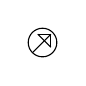
\begin{tikzpicture}
        \draw (0,0) circle (1.2ex);
        \draw (0.7 ex, 0.7 ex) -- (-0.4 ex, 0.7 ex);
        \draw (-0.4 ex, 0.7 ex) -- (0.7 ex, -0.4 ex);
        \draw (0.7 ex, -0.4 ex) -- (0.7 ex, 0.7 ex);
        \draw (0.7 ex, 0.7 ex) -- (-0.848 ex, -0.848 ex);
    \end{tikzpicture}}}
    \ \ 
}

% legendre符号
\makeatletter
\def\legendre@dash#1#2{\hb@xt@#1{%
  \kern-#2\p@
  \cleaders\hbox{\kern.5\p@
    \vrule\@height.2\p@\@depth.2\p@\@width\p@
    \kern.5\p@}\hfil
  \kern-#2\p@
  }}
\def\@legendre#1#2#3#4#5{\mathopen{}\left(
  \sbox\z@{$\genfrac{}{}{0pt}{#1}{#3#4}{#3#5}$}%
  \dimen@=\wd\z@
  \kern-\p@\vcenter{\box0}\kern-\dimen@\vcenter{\legendre@dash\dimen@{#2}}\kern-\p@
  \right)\mathclose{}}
\newcommand\legendre[2]{\mathchoice
  {\@legendre{0}{1}{}{#1}{#2}}
  {\@legendre{1}{.5}{\vphantom{1}}{#1}{#2}}
  {\@legendre{2}{0}{\vphantom{1}}{#1}{#2}}
  {\@legendre{3}{0}{\vphantom{1}}{#1}{#2}}
}
\def\dlegendre{\@legendre{0}{1}{}}
\def\tlegendre{\@legendre{1}{0.5}{\vphantom{1}}}
\makeatother





% 单一字母in mathbb mathcal mathsf mathrm mathfrak mathscr symbf symrm symup
\newcommand{\bbA}{{\mathbb{A}}}
\newcommand{\bba}{{\mathbb{a}}}
\newcommand{\bbB}{{\mathbb{B}}}
\newcommand{\bbb}{{\mathbb{b}}}
\newcommand{\bbC}{{\mathbb{C}}}
\newcommand{\bbc}{{\mathbb{c}}}
\newcommand{\bbD}{{\mathbb{D}}} 
\newcommand{\bbd}{{\mathbb{d}}}
\newcommand{\bbE}{{\mathbb{E}}}
\newcommand{\bbe}{{\mathbb{e}}}
\newcommand{\bbF}{{\mathbb{F}}}
\newcommand{\bbf}{{\mathbb{f}}}
\newcommand{\bbG}{{\mathbb{G}}}
\newcommand{\bbg}{{\mathbb{g}}}
\newcommand{\bbH}{{\mathbb{H}}}
\newcommand{\bbh}{{\mathbb{h}}}
\newcommand{\bbI}{{\mathbb{I}}}
\newcommand{\bbi}{{\mathbb{i}}}
\newcommand{\bbJ}{{\mathbb{J}}}
\newcommand{\bbj}{{\mathbb{j}}}
\newcommand{\bbK}{{\mathbb{K}}}
\newcommand{\bbk}{{\mathbb{k}}}
\newcommand{\bbL}{{\mathbb{L}}}
\newcommand{\bbl}{{\mathbb{l}}}
\newcommand{\bbM}{{\mathbb{M}}}
\newcommand{\bbm}{{\mathbb{m}}}
\newcommand{\bbN}{{\mathbb{N}}}
\newcommand{\bbn}{{\mathbb{n}}}
\newcommand{\bbO}{{\mathbb{O}}}
\newcommand{\bbo}{{\mathbb{o}}}
\newcommand{\bbP}{{\mathbb{P}}}
\newcommand{\bbp}{{\mathbb{p}}}
\newcommand{\bbQ}{{\mathbb{Q}}}
\newcommand{\bbq}{{\mathbb{q}}}
\newcommand{\bbR}{{\mathbb{R}}}
\newcommand{\bbr}{{\mathbb{r}}}
\newcommand{\bbS}{{\mathbb{S}}}
\newcommand{\bbs}{{\mathbb{s}}}
\newcommand{\bbT}{{\mathbb{T}}}
\newcommand{\bbt}{{\mathbb{t}}}
\newcommand{\bbU}{{\mathbb{U}}}
\newcommand{\bbu}{{\mathbb{u}}}
\newcommand{\bbV}{{\mathbb{V}}}
\newcommand{\bbv}{{\mathbb{v}}}
\newcommand{\bbW}{{\mathbb{W}}}
\newcommand{\bbw}{{\mathbb{w}}}
\newcommand{\bbX}{{\mathbb{X}}}
\newcommand{\bbx}{{\mathbb{x}}}
\newcommand{\bbY}{{\mathbb{Y}}}
\newcommand{\bby}{{\mathbb{y}}}
\newcommand{\bbZ}{{\mathbb{Z}}}
\newcommand{\bbz}{{\mathbb{z}}}
\newcommand{\bbone}{{\mathbb{1}}}

\newcommand{\calA}{{\mathcal{A}}}
\newcommand{\cala}{{\mathcal{a}}}
\newcommand{\calB}{{\mathcal{B}}}
\newcommand{\calb}{{\mathcal{b}}}
\newcommand{\calC}{{\mathcal{C}}}
\newcommand{\calc}{{\mathcal{c}}}
\newcommand{\calD}{{\mathcal{D}}}
\newcommand{\cald}{{\mathcal{d}}}
\newcommand{\calE}{{\mathcal{E}}}
\newcommand{\cale}{{\mathcal{e}}}
\newcommand{\calF}{{\mathcal{F}}}
\newcommand{\calf}{{\mathcal{f}}}
\newcommand{\calG}{{\mathcal{G}}}
\newcommand{\calg}{{\mathcal{g}}}
\newcommand{\calH}{{\mathcal{H}}}
\newcommand{\calh}{{\mathcal{h}}}
\newcommand{\calI}{{\mathcal{I}}}
\newcommand{\cali}{{\mathcal{i}}}
\newcommand{\calJ}{{\mathcal{J}}}
\newcommand{\calj}{{\mathcal{j}}}
\newcommand{\calK}{{\mathcal{K}}}
\newcommand{\calk}{{\mathcal{k}}}
\newcommand{\calL}{{\mathcal{L}}}
\newcommand{\call}{{\mathcal{l}}}
\newcommand{\calM}{{\mathcal{M}}}
\newcommand{\calm}{{\mathcal{m}}}
\newcommand{\calN}{{\mathcal{N}}}
\newcommand{\caln}{{\mathcal{n}}}
\newcommand{\calO}{{\mathcal{O}}}
\newcommand{\calo}{{\mathcal{o}}}
\newcommand{\calP}{{\mathcal{P}}}
\newcommand{\calp}{{\mathcal{p}}}
\newcommand{\calQ}{{\mathcal{Q}}}
\newcommand{\calq}{{\mathcal{q}}}
\newcommand{\calR}{{\mathcal{R}}}
\newcommand{\calr}{{\mathcal{r}}}
\newcommand{\calS}{{\mathcal{S}}}
\newcommand{\cals}{{\mathcal{s}}}
\newcommand{\calT}{{\mathcal{T}}}
\newcommand{\calt}{{\mathcal{t}}}
\newcommand{\calU}{{\mathcal{U}}}
\newcommand{\calu}{{\mathcal{u}}}
\newcommand{\calV}{{\mathcal{V}}}
\newcommand{\calv}{{\mathcal{v}}}
\newcommand{\calW}{{\mathcal{W}}}
\newcommand{\calw}{{\mathcal{w}}}
\newcommand{\calX}{{\mathcal{X}}}
\newcommand{\calx}{{\mathcal{x}}}
\newcommand{\calY}{{\mathcal{Y}}}
\newcommand{\caly}{{\mathcal{y}}}
\newcommand{\calZ}{{\mathcal{Z}}}
\newcommand{\calz}{{\mathcal{z}}}

\newcommand{\scrA}{{\mathscr{A}}}
\newcommand{\scra}{{\mathscr{a}}}
\newcommand{\scrB}{{\mathscr{B}}}
\newcommand{\scrb}{{\mathscr{b}}}
\newcommand{\scrC}{{\mathscr{C}}}
\newcommand{\scrc}{{\mathscr{c}}}
\newcommand{\scrD}{{\mathscr{D}}}
\newcommand{\scrd}{{\mathscr{d}}}
\newcommand{\scrE}{{\mathscr{E}}}
\newcommand{\scre}{{\mathscr{e}}}
\newcommand{\scrF}{{\mathscr{F}}}
\newcommand{\scrf}{{\mathscr{f}}}
\newcommand{\scrG}{{\mathscr{G}}}
\newcommand{\scrg}{{\mathscr{g}}}
\newcommand{\scrH}{{\mathscr{H}}}
\newcommand{\scrh}{{\mathscr{h}}}
\newcommand{\scrI}{{\mathscr{I}}}
\newcommand{\scri}{{\mathscr{i}}}
\newcommand{\scrJ}{{\mathscr{J}}}
\newcommand{\scrj}{{\mathscr{j}}}
\newcommand{\scrK}{{\mathscr{K}}}
\newcommand{\scrk}{{\mathscr{k}}}
\newcommand{\scrL}{{\mathscr{L}}}
\newcommand{\scrl}{{\mathscr{l}}}
\newcommand{\scrM}{{\mathscr{M}}}
\newcommand{\scrm}{{\mathscr{m}}}
\newcommand{\scrN}{{\mathscr{N}}}
\newcommand{\scrn}{{\mathscr{n}}}
\newcommand{\scrO}{{\mathscr{O}}}
\newcommand{\scro}{{\mathscr{o}}}
\newcommand{\scrP}{{\mathscr{P}}}
\newcommand{\scrp}{{\mathscr{p}}}
\newcommand{\scrQ}{{\mathscr{Q}}}
\newcommand{\scrq}{{\mathscr{q}}}
\newcommand{\scrR}{{\mathscr{R}}}
\newcommand{\scrr}{{\mathscr{r}}}
\newcommand{\scrS}{{\mathscr{S}}}
\newcommand{\scrs}{{\mathscr{s}}}
\newcommand{\scrT}{{\mathscr{T}}}
\newcommand{\scrt}{{\mathscr{t}}}
\newcommand{\scrU}{{\mathscr{U}}}
\newcommand{\scru}{{\mathscr{u}}}
\newcommand{\scrV}{{\mathscr{V}}}
\newcommand{\scrv}{{\mathscr{v}}}
\newcommand{\scrW}{{\mathscr{W}}}
\newcommand{\scrw}{{\mathscr{w}}}
\newcommand{\scrX}{{\mathscr{X}}}
\newcommand{\scrx}{{\mathscr{x}}}
\newcommand{\scrY}{{\mathscr{Y}}}
\newcommand{\scry}{{\mathscr{y}}}
\newcommand{\scrZ}{{\mathscr{Z}}}
\newcommand{\scrz}{{\mathscr{z}}}

\newcommand{\frakA}{{\mathfrak{A}}}
\newcommand{\fraka}{{\mathfrak{a}}}
\newcommand{\frakB}{{\mathfrak{B}}}
\newcommand{\frakb}{{\mathfrak{b}}}
\newcommand{\frakC}{{\mathfrak{C}}}
\newcommand{\frakc}{{\mathfrak{c}}}
\newcommand{\frakD}{{\mathfrak{D}}}
\newcommand{\frakd}{{\mathfrak{d}}}
\newcommand{\frakE}{{\mathfrak{E}}}
\newcommand{\frake}{{\mathfrak{e}}}
\newcommand{\frakF}{{\mathfrak{F}}}
\newcommand{\frakf}{{\mathfrak{f}}}
\newcommand{\frakG}{{\mathfrak{G}}}
\newcommand{\frakg}{{\mathfrak{g}}}
\newcommand{\frakH}{{\mathfrak{H}}}
\newcommand{\frakh}{{\mathfrak{h}}}
\newcommand{\frakI}{{\mathfrak{I}}}
\newcommand{\fraki}{{\mathfrak{i}}}
\newcommand{\frakJ}{{\mathfrak{J}}}
\newcommand{\frakj}{{\mathfrak{j}}}
\newcommand{\frakK}{{\mathfrak{K}}}
\newcommand{\frakk}{{\mathfrak{k}}}
\newcommand{\frakL}{{\mathfrak{L}}}
\newcommand{\frakl}{{\mathfrak{l}}}
\newcommand{\frakM}{{\mathfrak{M}}}
\newcommand{\frakm}{{\mathfrak{m}}}
\newcommand{\frakN}{{\mathfrak{N}}}
\newcommand{\frakn}{{\mathfrak{n}}}
\newcommand{\frakO}{{\mathfrak{O}}}
\newcommand{\frako}{{\mathfrak{o}}}
\newcommand{\frakP}{{\mathfrak{P}}}
\newcommand{\frakp}{{\mathfrak{p}}}
\newcommand{\frakQ}{{\mathfrak{Q}}}
\newcommand{\frakq}{{\mathfrak{q}}}
\newcommand{\frakR}{{\mathfrak{R}}}
\newcommand{\frakr}{{\mathfrak{r}}}
\newcommand{\frakS}{{\mathfrak{S}}}
\newcommand{\fraks}{{\mathfrak{s}}}
\newcommand{\frakT}{{\mathfrak{T}}}
\newcommand{\frakt}{{\mathfrak{t}}}
\newcommand{\frakU}{{\mathfrak{U}}}
\newcommand{\fraku}{{\mathfrak{u}}}
\newcommand{\frakV}{{\mathfrak{V}}}
\newcommand{\frakv}{{\mathfrak{v}}}
\newcommand{\frakW}{{\mathfrak{W}}}
\newcommand{\frakw}{{\mathfrak{w}}}
\newcommand{\frakX}{{\mathfrak{X}}}
\newcommand{\frakx}{{\mathfrak{x}}}
\newcommand{\frakY}{{\mathfrak{Y}}}
\newcommand{\fraky}{{\mathfrak{y}}}
\newcommand{\frakZ}{{\mathfrak{Z}}}
\newcommand{\frakz}{{\mathfrak{z}}}

\newcommand{\rmA}{{\symrm{A}}}
\newcommand{\rma}{{\symrm{a}}}
\newcommand{\rmB}{{\symrm{B}}}
\newcommand{\rmb}{{\symrm{b}}}
\newcommand{\rmC}{{\symrm{C}}}
\newcommand{\rmc}{{\symrm{c}}}
\newcommand{\rmD}{{\symrm{D}}}
\newcommand{\rmd}{{\symrm{d}}}
\newcommand{\rmE}{{\symrm{E}}}
\newcommand{\rme}{{\symrm{e}}}
\newcommand{\rmF}{{\symrm{F}}}
\newcommand{\rmf}{{\symrm{f}}}
\newcommand{\rmG}{{\symrm{G}}}
\newcommand{\rmg}{{\symrm{g}}}
\newcommand{\rmH}{{\symrm{H}}}
\newcommand{\rmh}{{\symrm{h}}}
\newcommand{\rmI}{{\symrm{I}}}
\newcommand{\rmi}{{\symrm{i}}}
\newcommand{\rmJ}{{\symrm{J}}}
\newcommand{\rmj}{{\symrm{j}}}
\newcommand{\rmK}{{\symrm{K}}}
\newcommand{\rmk}{{\symrm{k}}}
\newcommand{\rmL}{{\symrm{L}}}
\newcommand{\rml}{{\symrm{l}}}
\newcommand{\rmM}{{\symrm{M}}}
\newcommand{\rmm}{{\symrm{m}}}
\newcommand{\rmN}{{\symrm{N}}}
\newcommand{\rmn}{{\symrm{n}}}
\newcommand{\rmO}{{\symrm{O}}}
\newcommand{\rmo}{{\symrm{o}}}
\newcommand{\rmP}{{\symrm{P}}}
\newcommand{\rmp}{{\symrm{p}}}
\newcommand{\rmQ}{{\symrm{Q}}}
\newcommand{\rmq}{{\symrm{q}}}
\newcommand{\rmR}{{\symrm{R}}}
\newcommand{\rmr}{{\symrm{r}}}
\newcommand{\rmS}{{\symrm{S}}}
\newcommand{\rms}{{\symrm{s}}}
\newcommand{\rmT}{{\symrm{T}}}
\newcommand{\rmt}{{\symrm{t}}}
\newcommand{\rmU}{{\symrm{U}}}
\newcommand{\rmu}{{\symrm{u}}}
\newcommand{\rmV}{{\symrm{V}}}
\newcommand{\rmv}{{\symrm{v}}}
\newcommand{\rmW}{{\symrm{W}}}
\newcommand{\rmw}{{\symrm{w}}}
\newcommand{\rmX}{{\symrm{X}}}
\newcommand{\rmx}{{\symrm{x}}}
\newcommand{\rmY}{{\symrm{Y}}}
\newcommand{\rmy}{{\symrm{y}}}
\newcommand{\rmZ}{{\symrm{Z}}}
\newcommand{\rmz}{{\symrm{z}}}

\newcommand{\upA}{{\symup{A}}}
\newcommand{\upa}{{\symup{a}}}
\newcommand{\upB}{{\symup{B}}}
\newcommand{\upb}{{\symup{b}}}
\newcommand{\upC}{{\symup{C}}}
\newcommand{\upc}{{\symup{c}}}
\newcommand{\upD}{{\symup{D}}}
\newcommand{\upd}{{\symup{d}}}
\newcommand{\upE}{{\symup{E}}}
\newcommand{\upe}{{\symup{e}}}
\newcommand{\upF}{{\symup{F}}}
\newcommand{\upf}{{\symup{f}}}
\newcommand{\upG}{{\symup{G}}}
\newcommand{\upg}{{\symup{g}}}
\newcommand{\upH}{{\symup{H}}}
\newcommand{\uph}{{\symup{h}}}
\newcommand{\upI}{{\symup{I}}}
\newcommand{\upi}{{\symup{i}}}
\newcommand{\upJ}{{\symup{J}}}
\newcommand{\upj}{{\symup{j}}}
\newcommand{\upK}{{\symup{K}}}
\newcommand{\upk}{{\symup{k}}}
\newcommand{\upL}{{\symup{L}}}
\newcommand{\upl}{{\symup{l}}}
\newcommand{\upM}{{\symup{M}}}
\newcommand{\upm}{{\symup{m}}}
\newcommand{\upN}{{\symup{N}}}
\newcommand{\upn}{{\symup{n}}}
\newcommand{\upO}{{\symup{O}}}
\newcommand{\upo}{{\symup{o}}}
\newcommand{\upP}{{\symup{P}}}
\newcommand{\upp}{{\symup{p}}}
\newcommand{\upQ}{{\symup{Q}}}
\newcommand{\upq}{{\symup{q}}}
\newcommand{\upR}{{\symup{R}}}
\newcommand{\upr}{{\symup{r}}}
\newcommand{\upS}{{\symup{S}}}
\newcommand{\ups}{{\symup{s}}}
\newcommand{\upT}{{\symup{T}}}
\newcommand{\upt}{{\symup{t}}}
\newcommand{\upU}{{\symup{U}}}
\newcommand{\upu}{{\symup{u}}}
\newcommand{\upV}{{\symup{V}}}
\newcommand{\upv}{{\symup{v}}}
\newcommand{\upW}{{\symup{W}}}
\newcommand{\upw}{{\symup{w}}}
\newcommand{\upX}{{\symup{X}}}
\newcommand{\upx}{{\symup{x}}}
\newcommand{\upY}{{\symup{Y}}}
\newcommand{\upy}{{\symup{y}}}
\newcommand{\upZ}{{\symup{Z}}}
\newcommand{\upz}{{\symup{z}}}

\newcommand{\bfA}{{\symbf{A}}}
\newcommand{\bfa}{{\symbf{a}}}
\newcommand{\bfB}{{\symbf{B}}}
\newcommand{\bfb}{{\symbf{b}}}
\newcommand{\bfC}{{\symbf{C}}}
\newcommand{\bfc}{{\symbf{c}}}
\newcommand{\bfD}{{\symbf{D}}}
\newcommand{\bfd}{{\symbf{d}}}
\newcommand{\bfE}{{\symbf{E}}}
\newcommand{\bfe}{{\symbf{e}}}
\newcommand{\bfF}{{\symbf{F}}}
\newcommand{\bff}{{\symbf{f}}}
\newcommand{\bfG}{{\symbf{G}}}
\newcommand{\bfg}{{\symbf{g}}}
\newcommand{\bfH}{{\symbf{H}}}
\newcommand{\bfh}{{\symbf{h}}}
\newcommand{\bfI}{{\symbf{I}}}
\newcommand{\bfi}{{\symbf{i}}}
\newcommand{\bfJ}{{\symbf{J}}}
\newcommand{\bfj}{{\symbf{j}}}
\newcommand{\bfK}{{\symbf{K}}}
\newcommand{\bfk}{{\symbf{k}}}
\newcommand{\bfL}{{\symbf{L}}}
\newcommand{\bfl}{{\symbf{l}}}
\newcommand{\bfM}{{\symbf{M}}}
\newcommand{\bfm}{{\symbf{m}}}
\newcommand{\bfN}{{\symbf{N}}}
\newcommand{\bfn}{{\symbf{n}}}
\newcommand{\bfO}{{\symbf{O}}}
\newcommand{\bfo}{{\symbf{o}}}
\newcommand{\bfP}{{\symbf{P}}}
\newcommand{\bfp}{{\symbf{p}}}
\newcommand{\bfQ}{{\symbf{Q}}}
\newcommand{\bfq}{{\symbf{q}}}
\newcommand{\bfR}{{\symbf{R}}}
\newcommand{\bfr}{{\symbf{r}}}
\newcommand{\bfS}{{\symbf{S}}}
\newcommand{\bfs}{{\symbf{s}}}
\newcommand{\bfT}{{\symbf{T}}}
\newcommand{\bft}{{\symbf{t}}}
\newcommand{\bfU}{{\symbf{U}}}
\newcommand{\bfu}{{\symbf{u}}}
\newcommand{\bfV}{{\symbf{V}}}
\newcommand{\bfv}{{\symbf{v}}}
\newcommand{\bfW}{{\symbf{W}}}
\newcommand{\bfw}{{\symbf{w}}}
\newcommand{\bfX}{{\symbf{X}}}
\newcommand{\bfx}{{\symbf{x}}}
\newcommand{\bfY}{{\symbf{Y}}}
\newcommand{\bfy}{{\symbf{y}}}
\newcommand{\bfZ}{{\symbf{Z}}}
\newcommand{\bfz}{{\symbf{z}}}

\newcommand{\sfA}{{\mathsf{A}}}
\newcommand{\sfa}{{\mathsf{a}}}
\newcommand{\sfB}{{\mathsf{B}}}
\newcommand{\sfb}{{\mathsf{b}}}
\newcommand{\sfC}{{\mathsf{C}}}
\newcommand{\sfc}{{\mathsf{c}}}
\newcommand{\sfD}{{\mathsf{D}}}
\newcommand{\sfd}{{\mathsf{d}}}
\newcommand{\sfE}{{\mathsf{E}}}
\newcommand{\sfe}{{\mathsf{e}}}
\newcommand{\sfF}{{\mathsf{F}}}
\newcommand{\sff}{{\mathsf{f}}}
\newcommand{\sfG}{{\mathsf{G}}}
\newcommand{\sfg}{{\mathsf{g}}}
\newcommand{\sfH}{{\mathsf{H}}}
\newcommand{\sfh}{{\mathsf{h}}}
\newcommand{\sfI}{{\mathsf{I}}}
\newcommand{\sfi}{{\mathsf{i}}}
\newcommand{\sfJ}{{\mathsf{J}}}
\newcommand{\sfj}{{\mathsf{j}}}
\newcommand{\sfK}{{\mathsf{K}}}
\newcommand{\sfk}{{\mathsf{k}}}
\newcommand{\sfL}{{\mathsf{L}}}
\newcommand{\sfl}{{\mathsf{l}}}
\newcommand{\sfM}{{\mathsf{M}}}
\newcommand{\sfm}{{\mathsf{m}}}
\newcommand{\sfN}{{\mathsf{N}}}
\newcommand{\sfn}{{\mathsf{n}}}
\newcommand{\sfO}{{\mathsf{O}}}
\newcommand{\sfo}{{\mathsf{o}}}
\newcommand{\sfP}{{\mathsf{P}}}
\newcommand{\sfp}{{\mathsf{p}}}
\newcommand{\sfQ}{{\mathsf{Q}}}
\newcommand{\sfq}{{\mathsf{q}}}
\newcommand{\sfR}{{\mathsf{R}}}
\newcommand{\sfr}{{\mathsf{r}}}
\newcommand{\sfS}{{\mathsf{S}}}
\newcommand{\sfs}{{\mathsf{s}}}
\newcommand{\sfT}{{\mathsf{T}}}
\newcommand{\sft}{{\mathsf{t}}}
\newcommand{\sfU}{{\mathsf{U}}}
\newcommand{\sfu}{{\mathsf{u}}}
\newcommand{\sfV}{{\mathsf{V}}}
\newcommand{\sfv}{{\mathsf{v}}}
\newcommand{\sfW}{{\mathsf{W}}}
\newcommand{\sfw}{{\mathsf{w}}}
\newcommand{\sfX}{{\mathsf{X}}}
\newcommand{\sfx}{{\mathsf{x}}}
\newcommand{\sfY}{{\mathsf{Y}}}
\newcommand{\sfy}{{\mathsf{y}}}
\newcommand{\sfZ}{{\mathsf{Z}}}
\newcommand{\sfz}{{\mathsf{z}}}
             % 加载符号定义文件
\addbibresource{../Accessories/ref.bib}            % 添加参考文献文件


\title{Template for the class ``Note for Myself'' in sectionlevel=book}
\author{The author}
\date{\today}
\authorpage{\href{https://www.example.com}{example.com}}

% available on the mode "\sectionlevel=chapter" or "\sectionlevel=book".
\setCJKfamilyfont{lxgwwenkai}{LXGW WenKai} % 定义霞鹜文楷,若未安装,请去掉相关代码编译或使用其他字体
\coversentence{\CJKfamily{lxgwwenkai}阿巴阿巴阿巴阿巴阿巴阿巴阿巴阿巴阿巴阿巴阿巴阿巴阿巴阿巴阿巴阿巴阿巴阿巴阿巴阿巴阿巴阿巴阿巴阿巴阿巴阿巴阿巴阿巴阿巴阿巴阿巴阿巴!}
\coverimage{placeholder.jpg} % 封面图片
\covertitlefont{Allura} % 封面标题字体, 若未安装,请去掉相关代码编译或使用其他字体
% \coverlinecolor{red} % 封面线条颜色
% \covertextcolor{green} % 封面文字颜色

% available on the mode "\sectionlevel=book".
\authoremail{email}
\texsource{\href{https://github.com/MonkeyUnderMountain/TexTemplates}{github.com/MonkeyUnderMountain/TexTemplates}}
\version{}

\begin{document}

    \maketitle

    \tableofcontents % 生成目录

    \chapter{In sectionlevel=book}

        \section{Section name}

\subsection{Fonts in math mode}

    We use the unicode-math package to support Unicode math symbols. Below is a list of common math symbols, grouped by font/style, with their names:

    \begin{itemize}
        \item \textbf{Greek letters:} \(\Alpha, \Beta, \Gamma, \Delta, \Epsilon, \Zeta, \Eta, \Theta, \Iota, \Kappa, \Lambda, \Mu, \Nu, \Xi, \Omicron, \Pi, \Rho, \Sigma, \Tau, \Upsilon, \Phi, \Chi, \Psi, \Omega\); 
        \item \(\alpha, \beta, \gamma, \delta, \epsilon, \varepsilon, \zeta, \eta, \theta, \iota, \kappa, \lambda, \mu, \nu, \xi, \omicron, \pi, \rho, \sigma, \tau, \upsilon, \phi, \varphi, \chi, \psi, \omega\);
        \item \textbf{Numbers and operators:} \(0, 1, 2, 3, 4, 5, 6, 7, 8, 9, +, -, \times, \div, =, <, >, \leq, \geq\)
        \item \textbf{Common math symbols:} \(\infty, \partial, \nabla, \forall, \exists, \neg, \land, \lor, \implies, \iff, \subset, \subseteq, \supset, \supseteq, \cup, \cap, \setminus, \emptyset,\injmap,\surjmap,\ratmap,\invlim,\dirlim\);
        \item \textbf{Musical symbols:} \(\sharp, \flat, \natural\);
        \item \textbf{math italic:} \(A, B, C, D, E, F, G, H, I, J, K, L, M, N, O, P, Q, R, S, T, U, V, W, X, Y, Z\); 
        \item \(a, b, c, d, e, f, g, h, i, j, k, l, m, n, o, p, q, r, s, t, u, v, w, x, y, z\);
        \item \textbf{Calligraphic:} $\calA, \calB, \calC, \calD, \calE, \calF, \calG, \calH, \calI, \calJ, \calK, \calL, \calM, \calN, \calO, \calP, \calQ, \calR, \calS, \calT, \calU, \calV, \calW, \calX, \calY, \calZ$, 
        \item $\cala, \calb, \calc, \cald, \cale, \calf, \calg, \calh, \cali, \calj, \calk, \call, \calm, \caln, \calo, \calp, \calq, \calr, \cals, \calt, \calu, \calv, \calw, \calx, \caly, \calz$
        \item \textbf{Blackboard bold:} \(\bbA, \bbB, \bbC, \bbD, \bbE, \bbF, \bbG, \bbH, \bbI, \bbJ, \bbK, \bbL, \bbM, \bbN, \bbO, \bbP, \bbQ, \bbR, \bbS, \bbT, \bbU, \bbV, \bbW, \bbX, \bbY, \bbZ\);
        \item \(\bba, \bbb, \bbc, \bbd, \bbe, \bbf, \bbg, \bbh, \bbi, \bbj, \bbk, \bbl, \bbm, \bbn, \bbo, \bbp, \bbq, \bbr, \bbs, \bbt, \bbu, \bbv, \bbw, \bbx, \bby, \bbz\);
        \item \textbf{Fraktur:} \(\frakA, \frakB, \frakC, \frakD, \frakE, \frakF, \frakG, \frakH, \frakI, \frakJ, \frakK, \frakL, \frakM, \frakN, \frakO, \frakP, \frakQ, \frakR, \frakS, \frakT, \frakU, \frakV, \frakW, \frakX, \frakY, \frakZ\);
        \item \(\fraka, \frakb, \frakc, \frakd, \frake, \frakf, \frakg, \frakh, \fraki, \frakj, \frakk, \frakl, \frakm, \frakn, \frako, \frakp, \frakq, \frakr, \fraks, \frakt, \fraku, \frakv, \frakw, \frakx, \fraky, \frakz\);
        \item \textbf{Script:} \(\scrA, \scrB, \scrC, \scrD, \scrE, \scrF, \scrG, \scrH, \scrI, \scrJ, \scrK, \scrL, \scrM, \scrN, \scrO, \scrP, \scrQ, \scrR, \scrS, \scrT, \scrU, \scrV, \scrW, \scrX, \scrY, \scrZ\);
        \item \(\scra, \scrb, \scrc, \scrd, \scre, \scrf, \scrg, \scrh, \scri, \scrj, \scrk, \scrl, \scrm, \scrn, \scro, \scrp, \scrq, \scrr, \scrs, \scrt, \scru, \scrv, \scrw, \scrx, \scry, \scrz\);
        \item \textbf{Upright:} \(\upA, \upB, \upC, \upD, \upE, \upF, \upG, \upH, \upI, \upJ, \upK, \upL, \upM, \upN, \upO, \upP, \upQ, \upR, \upS, \upT, \upU, \upV, \upW, \upX, \upY, \upZ\);
        \item \(\upa, \upb, \upc, \upd, \upe, \upf, \upg, \uph, \upi, \upj, \upk, \upl, \upm, \upn, \upo, \upp, \upq, \upr, \ups, \upt, \upu, \upv, \upw, \upx, \upy, \upz\);
        \item \textbf{Bold :} \(\bfA, \bfB, \bfC, \bfD, \bfE, \bfF, \bfG, \bfH, \bfI, \bfJ, \bfK, \bfL, \bfM, \bfN, \bfO, \bfP, \bfQ, \bfR, \bfS, \bfT, \bfU, \bfV, \bfW, \bfX, \bfY, \bfZ\);
        \item \(\bfa, \bfb, \bfc, \bfd, \bfe, \bff, \bfg, \bfh, \bfi, \bfj, \bfk, \bfl, \bfm, \bfn, \bfo, \bfp, \bfq, \bfr, \bfs, \bft, \bfu, \bfv, \bfw, \bfx, \bfy, \bfz\).
        \item \textbf{Sans-serif:} \(\sfA, \sfB, \sfC, \sfD, \sfE, \sfF, \sfG, \sfH, \sfI, \sfJ, \sfK, \sfL, \sfM, \sfN, \sfO, \sfP, \sfQ, \sfR, \sfS, \sfT, \sfU, \sfV, \sfW, \sfX, \sfY, \sfZ\);
        \item \(\sfa, \sfb, \sfc, \sfd, \sfe, \sff, \sfg, \sfh, \sfi, \sfj, \sfk, \sfl, \sfm, \sfn, \sfo, \sfp, \sfq, \sfr, \sfs, \sft, \sfu, \sfv, \sfw, \sfx, \sfy, \sfz\);
        \item \textbf{Roman:} \(\rmA, \rmB, \rmC, \rmD, \rmE, \rmF, \rmG, \rmH, \rmI, \rmJ, \rmK, \rmL, \rmM, \rmN, \rmO, \rmP, \rmQ, \rmR, \rmS, \rmT, \rmU, \rmV, \rmW, \rmX, \rmY, \rmZ\);
        \item \(\rma, \rmb, \rmc, \rmd, \rme, \rmf, \rmg, \rmh, \rmi, \rmj, \rmk, \rml, \rmm, \rmn, \rmo, \rmp, \rmq, \rmr, \rms, \rmt, \rmu, \rmv, \rmw, \rmx, \rmy, \rmz\);
    \end{itemize}

\subsection{Theorems and definitions}
    
    There are two types of theorem environments, one is with background color, the other is without background color. 
    The following is a list of theorem environments supported by this template:

    \begin{definition}[this is a definition]
        A \emph{locally ringed space} is a pair \((X, \calO_X)\), where \(X\) is a topological space, and \(\calO_X\) is a sheaf of rings on \(X\), such that for every point \(x \in X\), the stalk \(\calO_{X,x}\) is a local ring.
    \end{definition}
    \begin{proposition}[this is a proposition]
        test 
    \end{proposition}
    \begin{proof}
        This is a proof environment, it is used to prove theorems, propositions, lemmas, corollaries, etc.
        We allow to use step environments inside the proof environment, such as:
        \begin{step}\label{step:1_in_proof_1}
            This is a step environment, it is used to break down the proof into smaller steps.
        \end{step}
        \begin{step}\label{step:2_in_proof_1}
            This is another step environment, it is used to break down the proof into smaller steps.
        \end{step}
        And the step environment should be used inside the proof environment.
        The proof environment will automatically end with a square box.
    \end{proof}
    
    \begin{theorem}[this is a theorem]
        test 
    \end{theorem}
    \begin{proof}
        This is a proof environment.
        The step environment is labelled in the proof environment.
        A new proof environment will refresh the step environment counter.
        \begin{step}\label{step:1_in_proof_2}
            Goal 1.
        \end{step}
        Proof of Goal 1.
        
        \begin{step}\label{step:2_in_proof_2}
            Goal 2.
        \end{step}
        Proof of Goal 2.

        Here we test the hyperlink to the step environment \cref{step:1_in_proof_1}.

        You can also use the claim environment to make a claim in the proof environment, such as:
        \begin{claim}\label{claim:1_in_proof_2}
            This is a claim environment, it is used to make a claim in the proof environment.
        \end{claim}
        And the claim environment should be used inside the proof environment.
    \end{proof}
    \begin{proof}[Proof of \cref{claim:1_in_proof_2}]
        This is a proof for the \cref{claim:1_in_proof_2}.
        Here we test the case environment.
        \begin{case}\label{case:1_in_proof_2}
            This is a case environment, it is used to break down the proof into smaller cases.
        \end{case}
        \begin{case}\label{case:2_in_proof_2}
            This is another case environment, it is used to break down the proof into smaller cases.
        \end{case}
        And the case environment should be used inside the proof environment.
    \end{proof}

    \begin{lemma}[this is a lemma]
        test
    \end{lemma}
    \begin{proof}
        Here we test case environment again.
        \begin{case}\label{case:1_in_proof_3} 
            This is a case environment, it is used to break down the proof into smaller cases.
        \end{case}
        \begin{case}\label{case:2_in_proof_3}
            This is another case environment, it is used to break down the proof into smaller cases.
        \end{case}
    \end{proof}

    \begin{corollary}[this is a corollary]
        test 
    \end{corollary}
    \begin{question}[this is a question]
        test
    \end{question}
    \begin{conjecture}[this is a conjecture]
        test
    \end{conjecture}

    \begin{example}[this is an example]
        test 
    \end{example}
    \begin{exercise}[this is an exercise]
        test
    \end{exercise}
    \begin{remark}[this is a remark]
        test
        Here we test the hyperlink to the case environment \cref{case:1_in_proof_2}.
    \end{remark}
    \begin{proof}[this is a proof]
        test
    \end{proof}


 % 这里是正文

        \subsection{sectionlevel=book}

        % In this mode, the section is the highest level, and usually there is only one section in the document. 
        % There is no title page, no table of contents, and no cover image.
        % All theorem and definition environments are labelled with a unique number, and the numbering is continuous throughout the document.

        In this mode, the chapter is the highest level.
        The section is the second level, and the subsection is the third level.
        The section is numbered with the chapter number, such as 1.1, 1.2, etc.
        There is a title page, a table of contents, and a cover image.
        All theorem and definition environments are labelled in the form of chapter.number, such as 1.1, 1.2, etc.

    \chapter{Test}

        Test references \cite{Har77}.


        \section{Test Section}

        \subsection{Test Subsection}

        Test plots:

        \begin{figure}[htbp]
            \begin{center}
                %LaTeX with PSTricks extensions
%%Creator: Inkscape 1.4.2 (f4327f4, 2025-05-13)
%%Please note this file requires PSTricks extensions
\psset{xunit=.5pt,yunit=.5pt,runit=.5pt}
\begin{pspicture}(244.32627761,185.4730513)
{
\newrgbcolor{curcolor}{0 0 0}
\pscustom[linewidth=2.89133995,linecolor=curcolor]
{
\newpath
\moveto(45.24711842,40.85337142)
\curveto(58.73584213,29.29160867)(72.22416184,17.73019192)(87.63938451,20.18261487)
\curveto(103.05460817,22.63503782)(120.3330078,39.04079346)(138.6184774,41.23856541)
\curveto(156.90395701,43.43633837)(175.9274666,31.39393663)(195.02151618,19.30687989)
}
}
{
\newrgbcolor{curcolor}{0 0 0}
\pscustom[linewidth=2.89133995,linecolor=curcolor]
{
\newpath
\moveto(194.96947579,134.3218524)
\curveto(176.22577619,146.23373414)(157.88139659,157.89184289)(139.60670698,155.71104194)
\curveto(121.33201738,153.53024099)(104.05361775,137.12448534)(88.55080709,134.5844754)
\curveto(73.04799942,132.04446645)(59.38423272,143.43093721)(45.72060401,154.81729496)
\lineto(46.00938501,92.5800903)
\curveto(59.76927471,80.94343956)(73.72458941,69.14151981)(89.17788207,71.63895976)
\curveto(104.63117774,74.1363997)(121.90957736,90.54215935)(140.10278697,92.9534513)
\curveto(158.29600658,95.36474224)(177.13634617,83.7462395)(196.04654576,72.08464975)
\closepath
}
}
{
\newrgbcolor{curcolor}{0 0 0}
\pscustom[linewidth=1.00156996,linecolor=curcolor]
{
\newpath
\moveto(118.11178745,71.86551935)
\lineto(118.11178745,46.84183989)
}
}
{
\newrgbcolor{curcolor}{0 0 0}
\pscustom[linewidth=1.00156996,linecolor=curcolor]
{
\newpath
\moveto(115.10707755,49.5961573)
\lineto(118.11178745,46.5914474)
\lineto(121.11649734,49.5961573)
}
}
\end{pspicture}

            \end{center}
        \end{figure}

        There are some test texts here, and some test equations:

    \printbibliography[heading=bibintoc, title={References}] % 打印参考文献
\end{document}